\chapter{Using color separation as a stellar characterization tool}\label{chap:4}
% TEXT ==========================================

In this chapter, we consider the scope of using color as a stellar characterization tool. We display the probability functions and color statistics from our data analysis in Chapter \ref{chap:3}. We discuss how these color can be used in upcoming and current large-scale astronomical surveys, and the viability of using this method for exoplanet characterization.

\section{Color probability density functions}

From Chapter \ref{chap:3}, we have a method of determining color likelihood given a specified spectral and luminosity class, and we can use this to predict luminosity classes in cases that are unknown. In this section we present the probability density functions derived from fitting to Student's t-distribution (Figures \ref{fig:periodic-pdf-jw1}, \ref{fig:periodic-pdf-jw2},\ref{fig:periodic-delta-jw1}, and \ref{fig:periodic-delta-jw2}). We note that the color separation is subtle but non-negligible, on the order of $\sim$0.10 and $\sim$0.14 magnitudes for \jwone and \jwtwo, respectively, for spectral types G0--K3. No significant difference is observed for other spectral sub-types.

\section{Applicability to modern surveys}
Therefore $J$ is just special, and it should be a subject of future work as to why $J$ band spectral features are gravity sensitive for GKM dwarfs ($J-K$ for M dwarfs) and $J-W_{1,2}$ for GK dwarfs.

We also note the importance the $J$-band is in differentiating between dwarfs from giants given its previously proved sensitivity for differentiating M dwarfs from GK dwarfs for $J-K$ (REF). The combination of this study with $J-W_{1,2}$ in being sensitive for GK dwarfs, and $J-K$ being sensitive for GKM stars suggests the presence of surface gravity sensitive lines in the $J$-band. Thus, there we suggest it is viable to search for gravity sensitive lines along these the $J$-band wavelength range.

We consider use in large-scale  surveys that include photometric observations such as LAMOST, RAVE, and upcoming LSST. While color can help determine luminosity class, our tool would not work unless there is also a reliable estimate of spectral type as well...

Add exoplanet characterization stuff?

% FIGURES ==========================================
\begin{figure}
    \centering
    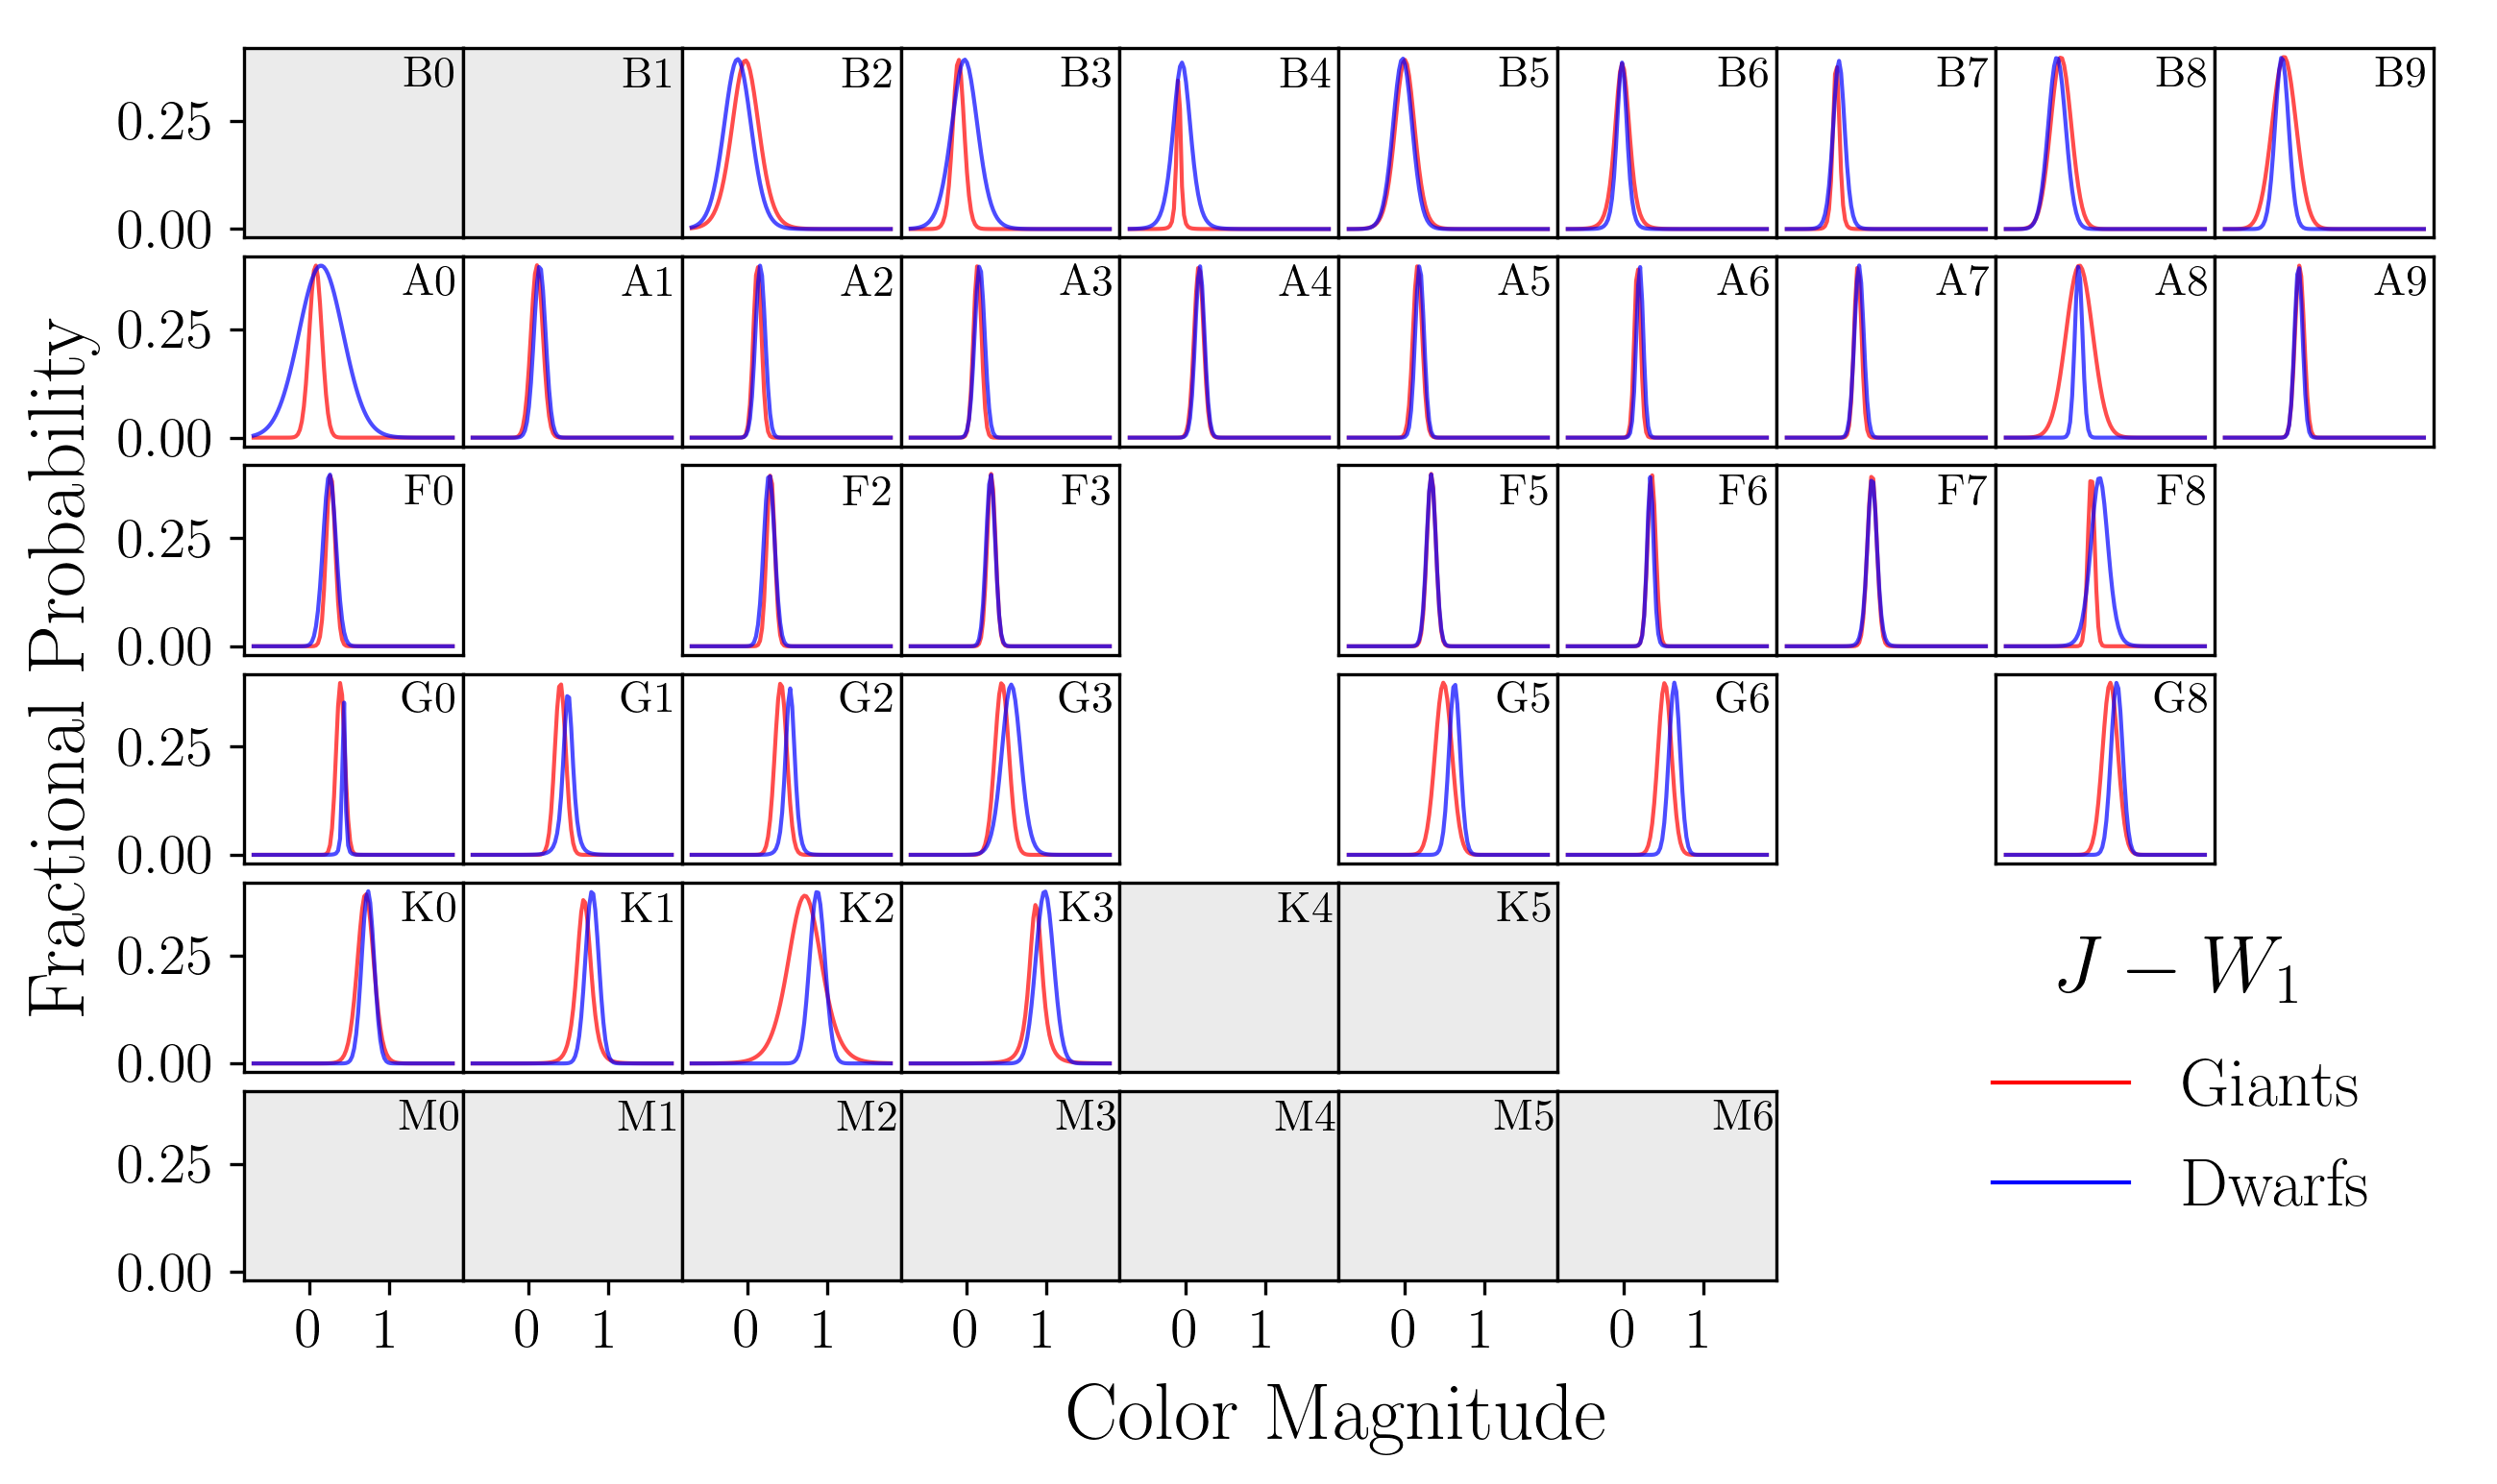
\includegraphics[width=1.0\textwidth,clip=true]{Figures/periodic/periodic-t-pdf_J_W1.png}
    \caption{This figure displays probability functions that are dependent on photometric color, spectral type, and luminosity class group (dwarfs and giants), from fitting photometric data to a Student's t distribution. We separated color data into luminosity and spectral class bins in order to detect any possible separation, or difference, in color amongst dwarfs from giants that are the same spectral type. There is a separation between dwarf and giant colors among spectral types G0 to K3. Grayed plots signify a spectral-type bin for which we do have some data, but have fewer than 4 stars in either luminosity group and thus cannot calculated an average. Spectral types not listed at all are types that are not represented in our $\sim$20,000 cross-matched sample from photometric and spectral catalogs, a process is described in Chapter \ref{chap:2}.}
    \label{fig:periodic-pdf-jw1}
\end{figure}

\begin{figure}
    \centering
    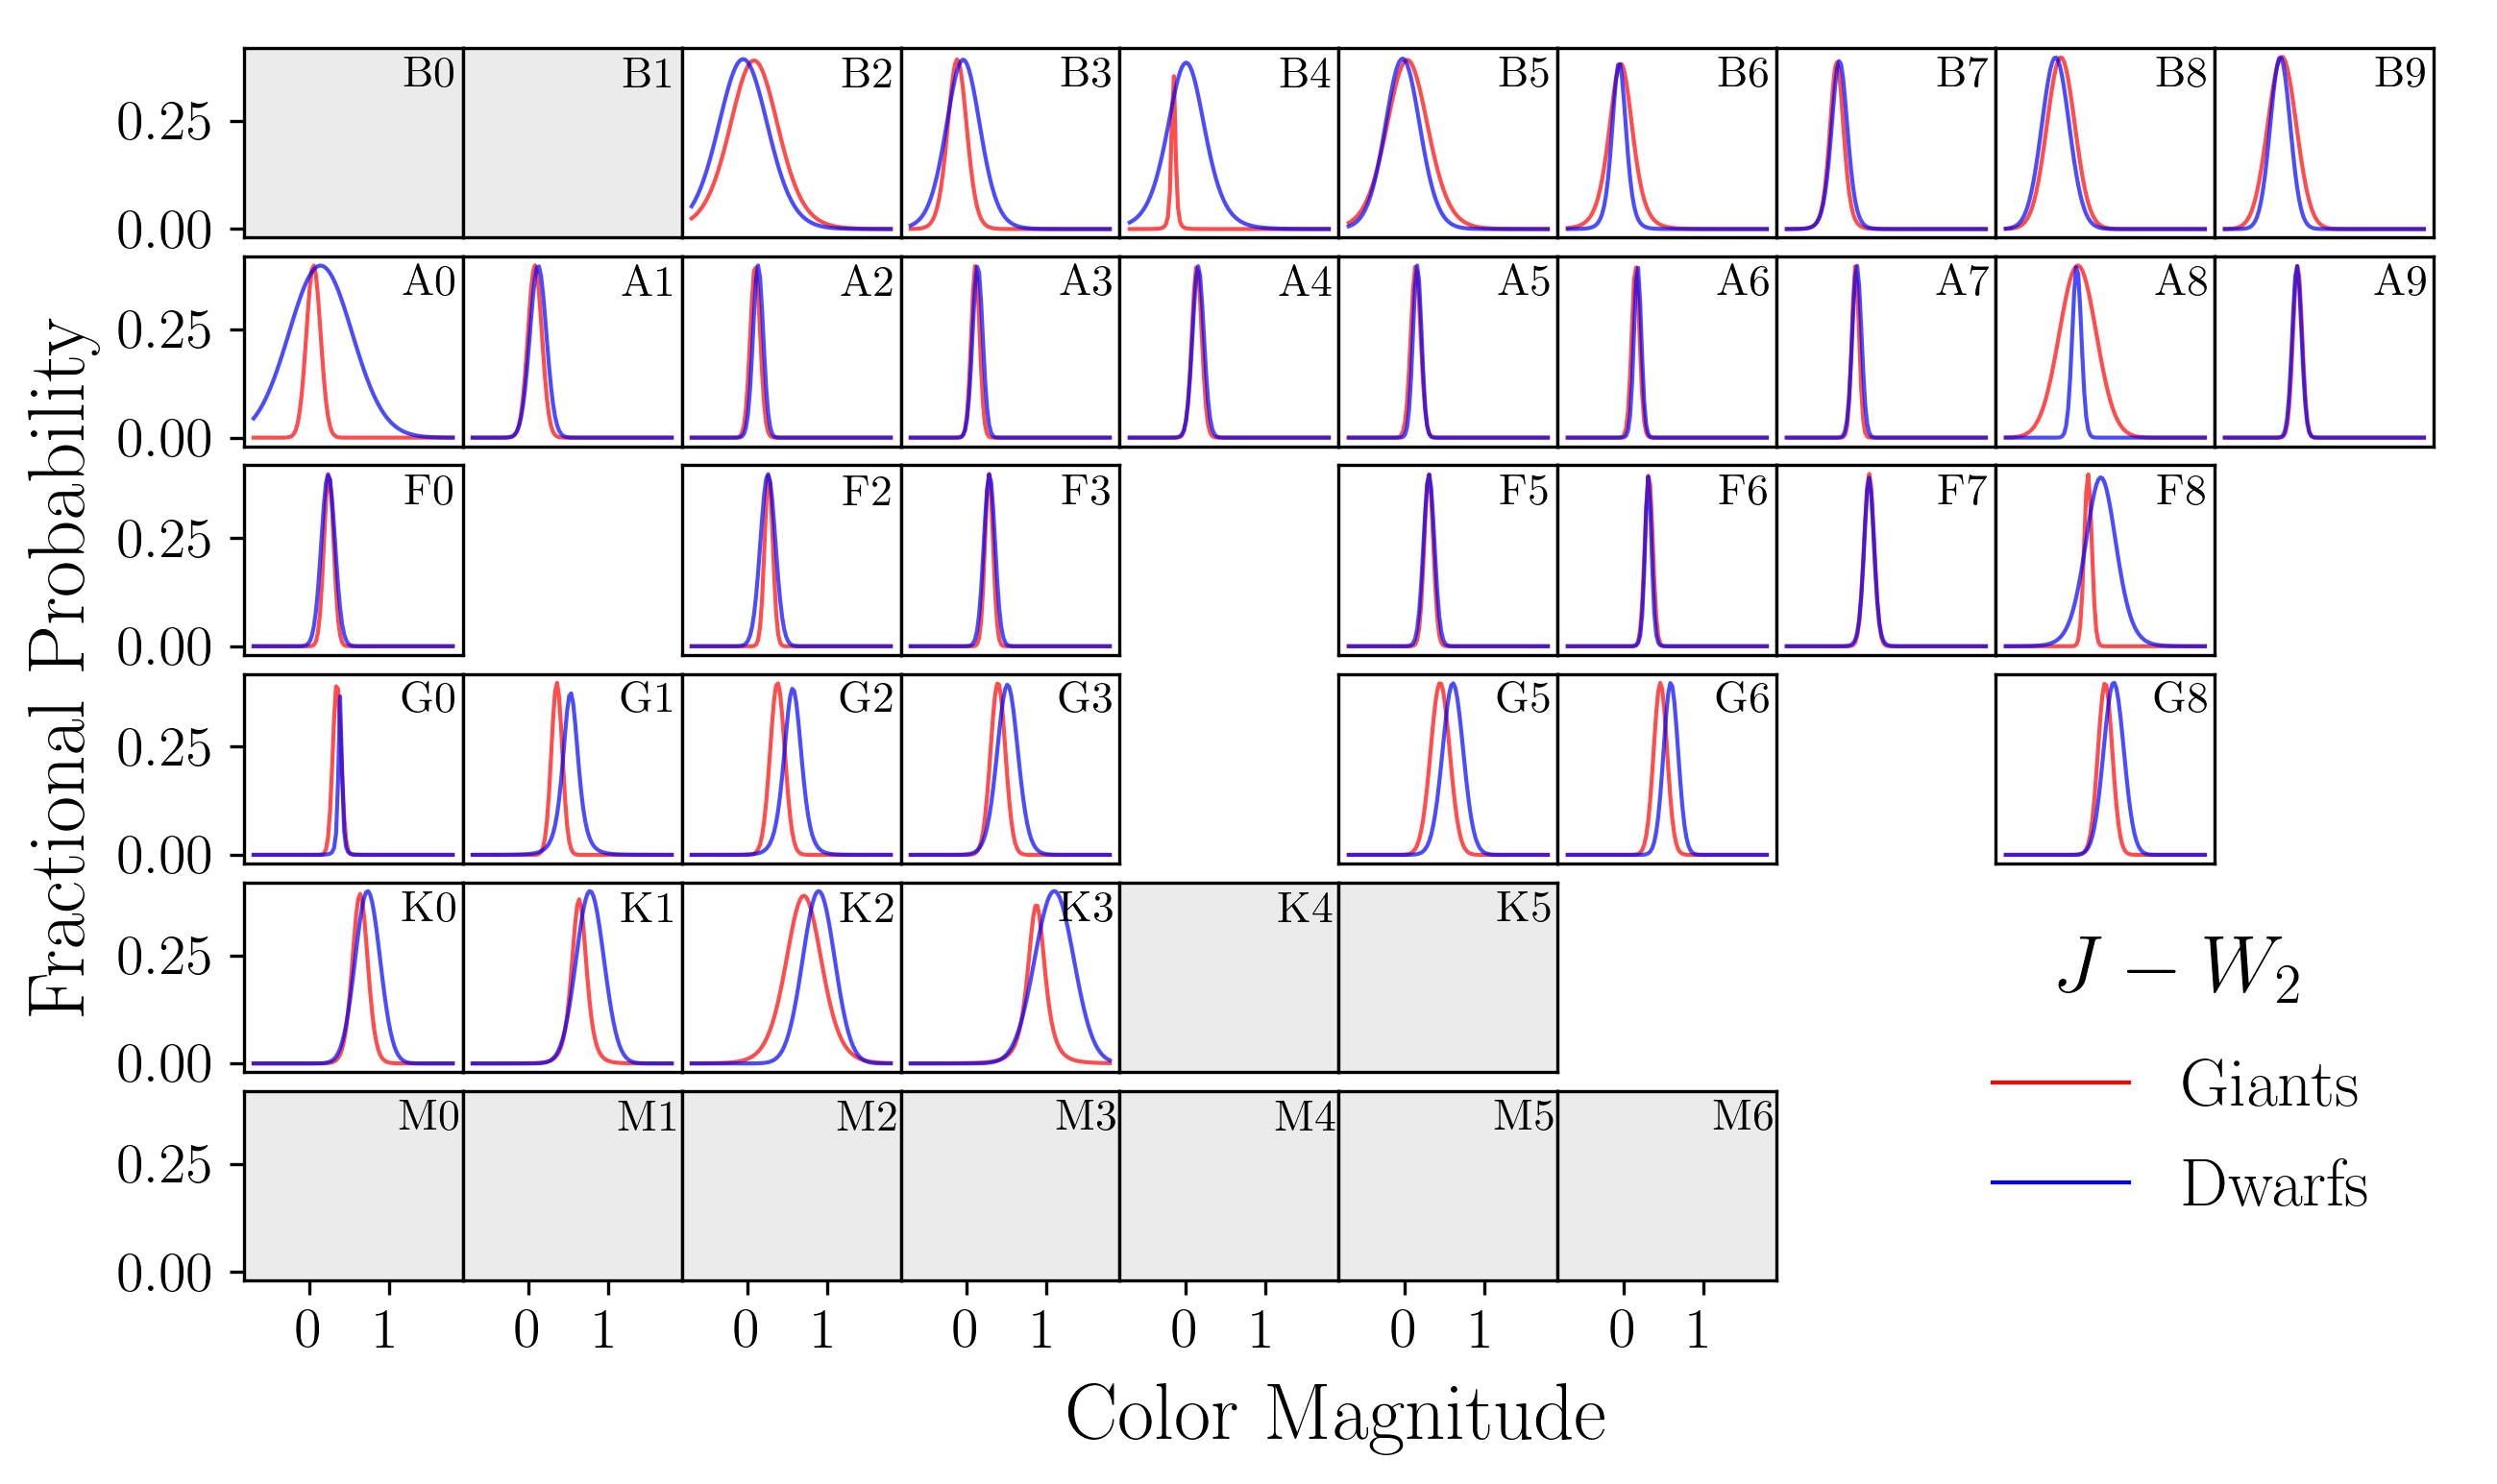
\includegraphics[width=1.0\textwidth,clip=true]{Figures/periodic/periodic-t-pdf_J_W2.png}
    \caption{Same as Figure \ref{fig:periodic-pdf-jw1}, but for \jwtwo.}
    \label{fig:periodic-pdf-jw2}
\end{figure}
\clearpage
\begin{figure}
    \centering
    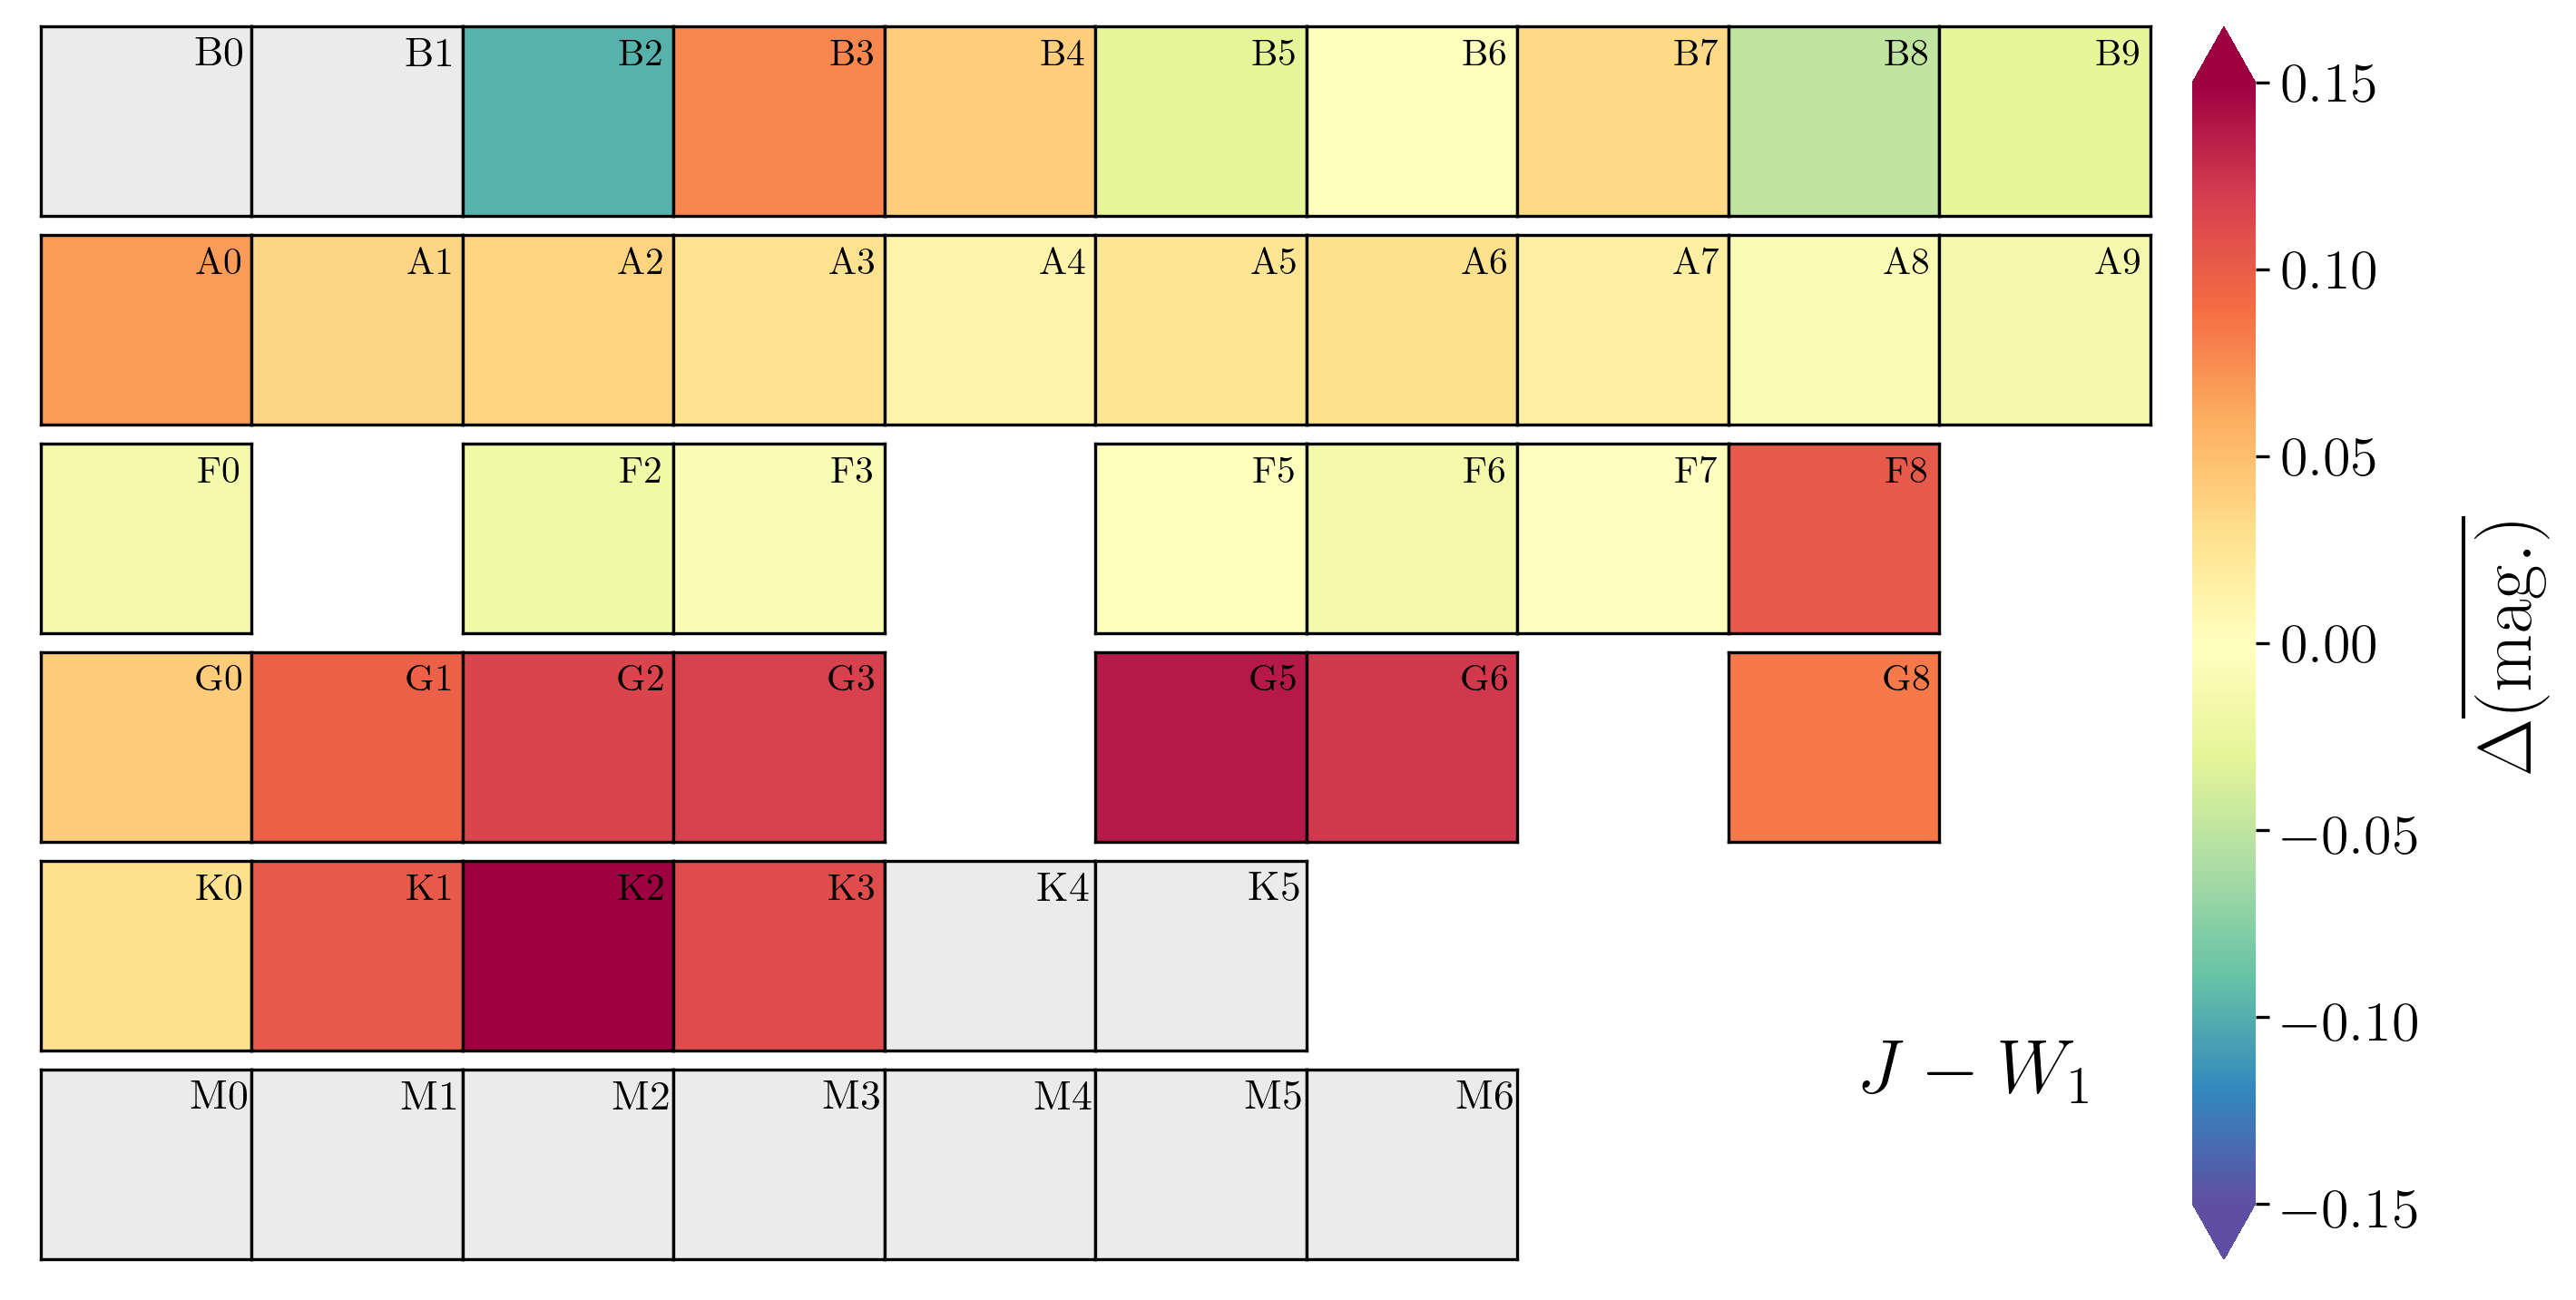
\includegraphics[width=1.0\textwidth,clip=true]{Figures/periodic/periodic-delta_J_W1.png}
    \caption{This figure is a derivative of Figures \ref{fig:periodic-pdf-jw1} and \ref{fig:periodic-pdf-jw2}, where we have simply subtracted color of the peak probability (or the average) of giants from dwarf luminosity groups for each spectral subtype bin. Presumably, the greater the difference in color, the easier it will be to differentiate giants from dwarfs of the same spectral type. This figure for \jwtwo, and the analogous figure for \jwtwo (Figure \ref{fig:periodic-delta-jw2}), highlights especially the spectral types for which we see the most color difference, G to early K-type stars.}
    \label{fig:periodic-delta-jw1}
\end{figure}

\begin{figure}
    \centering
    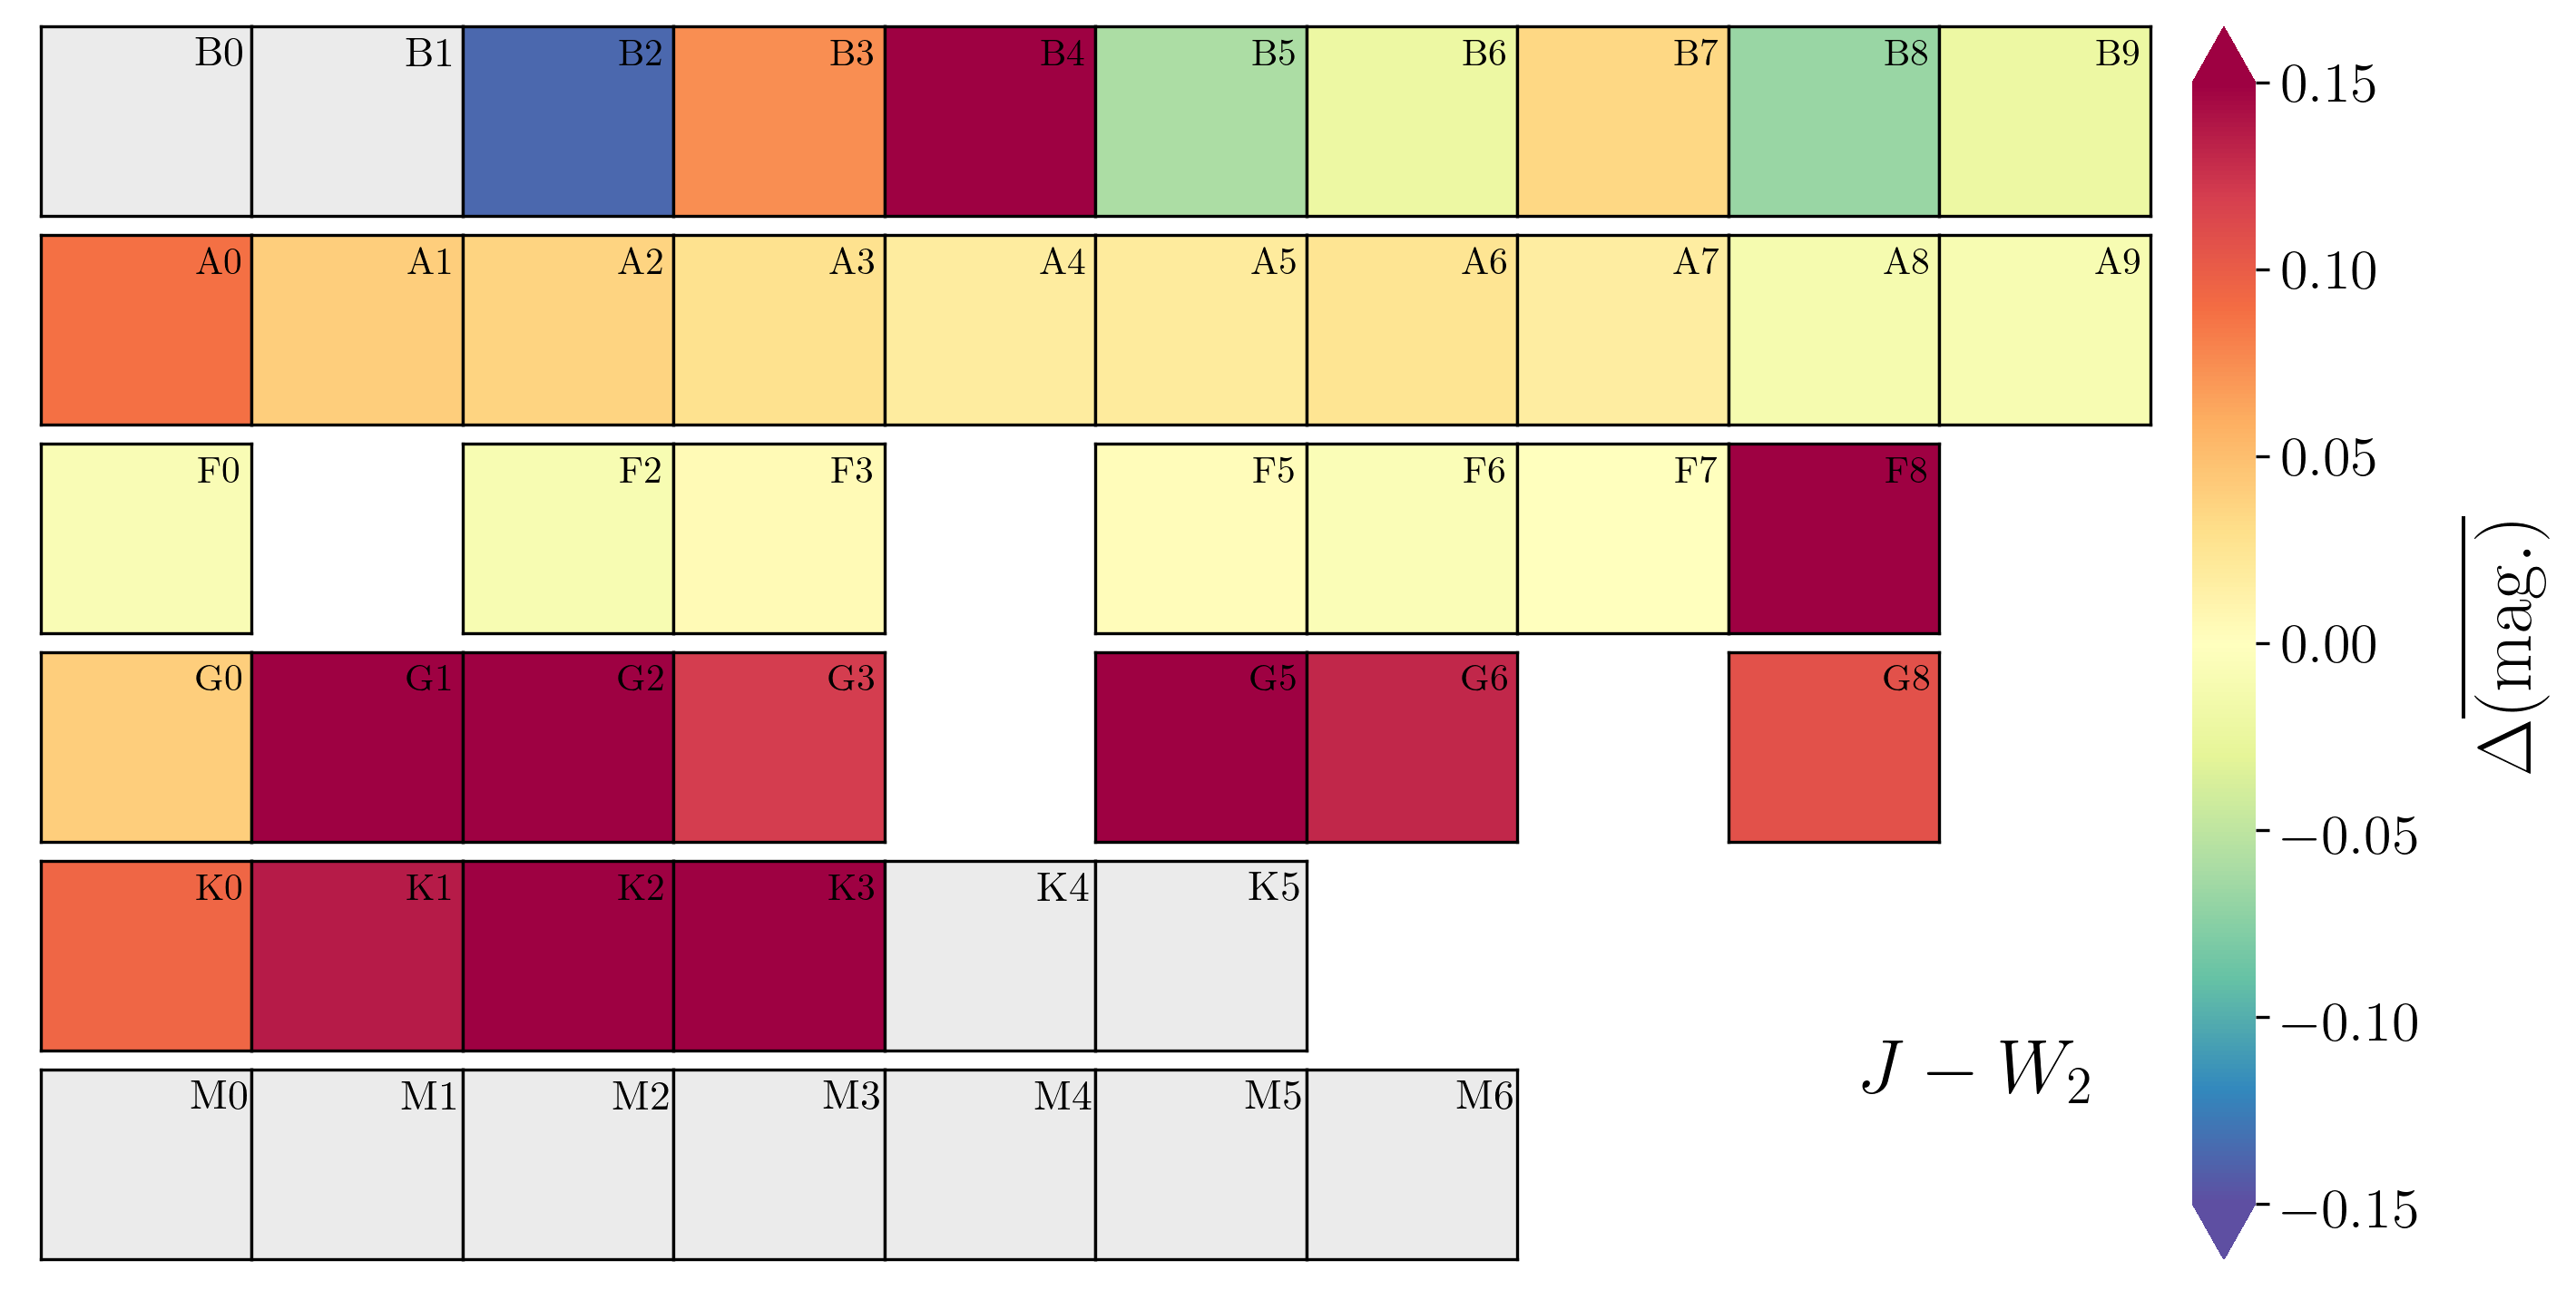
\includegraphics[width=1.0\textwidth,clip=true]{Figures/periodic/periodic-delta_J_W2.png}
    \caption{Same as Figure \ref{fig:periodic-delta-jw1}, but for \jwtwo.}
    \label{fig:periodic-delta-jw2}
\end{figure}
